\documentclass[cjk,10pt]{beamer}
\usepackage{CJK}
%\usepackage{beamerthemeshadow} %¸ÃΪһÏֳɵÄÄ£°å£¬ÔÚMiKTeX\texmf\tex\latex\beamer\themes\themeÏÂÃæÓкܶà
\usetheme{Warsaw}
\setbeamertemplate{headline}{}{}
\newcommand{\msize}{\scriptsize}
\usepackage{hyperref,amsmath,algorithm,algorithmic,multirow,xcolor}
\usepackage{amsthm,amsmath,enumerate,amsbsy,amsfonts,amssymb,mathabx,amscd,graphicx,algorithm}
\newtheorem{claim}{Claim}
\newtheorem{proposition}{Proposition}
\newtheorem{condition}{Condition}
\begin{document} %ÉêÃ÷ÎĵµµÄ¿ªÊ¼,
\begin{CJK*}{GBK}{song}     %CJK:Ö§³ÖÖÐÎÄ
\title{Report for Ovary data analysis}
\author{Xiaoqing Ye}
\institute{Institute of Statistics and Big Data}
\date{\today}
    \begin{frame} %beamerÀïÖØÒªµÄ¸ÅÄÿ¸öframe¶¨ÒåÒ»ÕÅpage
        \titlepage
    \end{frame}
    \begin{frame}
        \frametitle{Contents}
        \tableofcontents
    \end{frame}

    \section{Data description}
    \subsection{Data Structure}
    \begin{frame}
\begin{figure}[htbp]
\centering
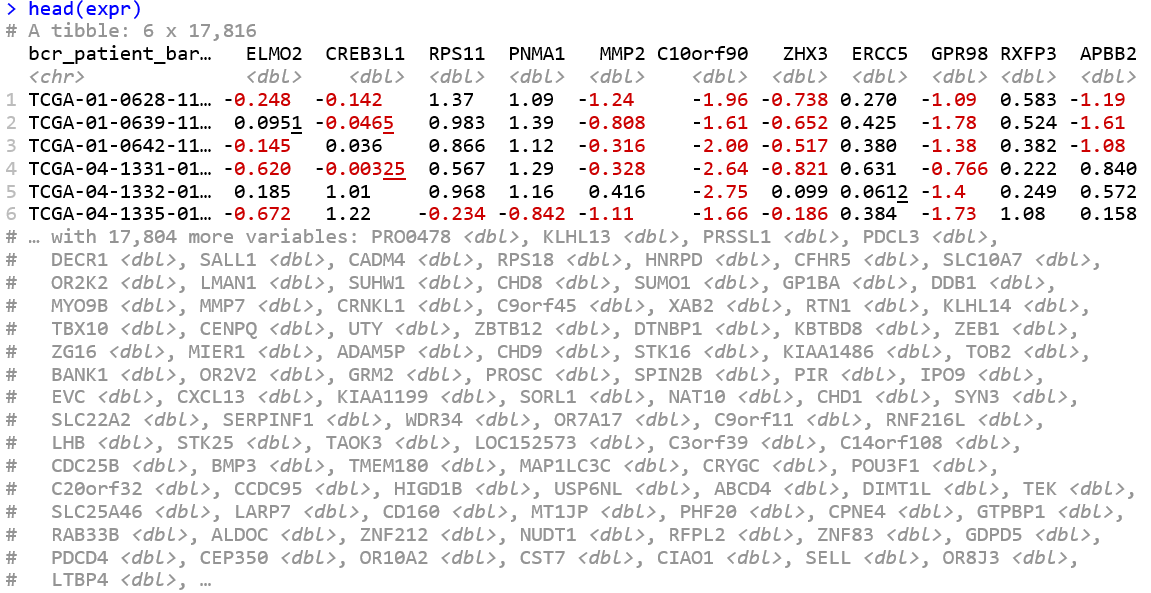
\includegraphics[height=5.5cm, width=8.5cm]{Yxq1as}
\caption{1}
\end{figure}


    \end{frame}
    \begin{frame}
\begin{figure}[htbp]
\centering
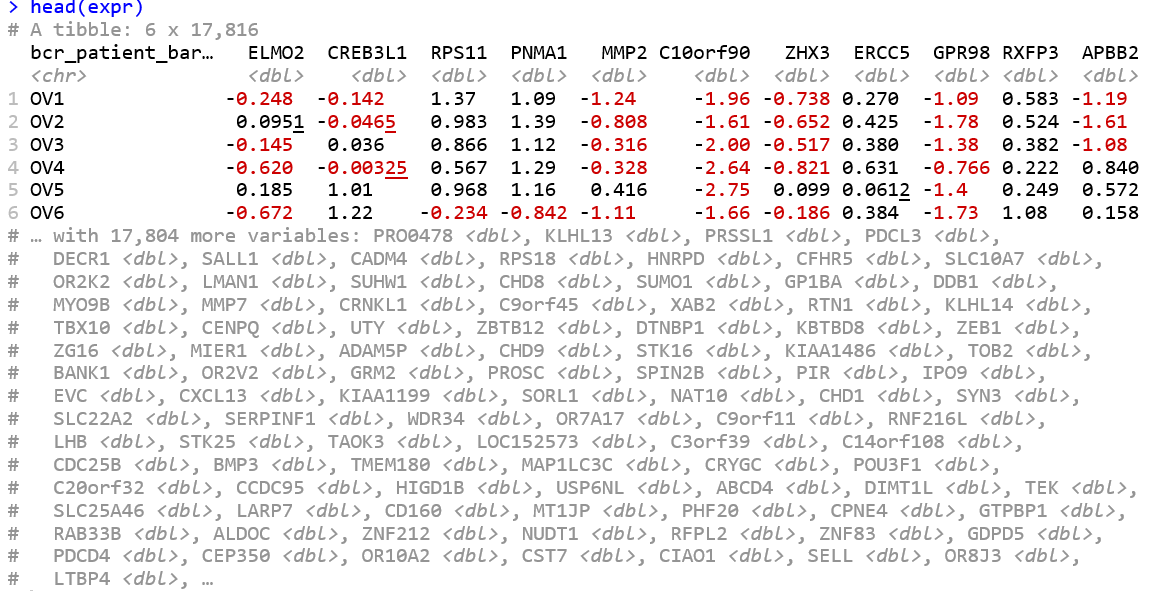
\includegraphics[height=5.5cm, width=8.5cm]{Yxq2as}
\caption{2}
\end{figure}


    \end{frame}
        \begin{frame}
\begin{figure}[htbp]
\centering
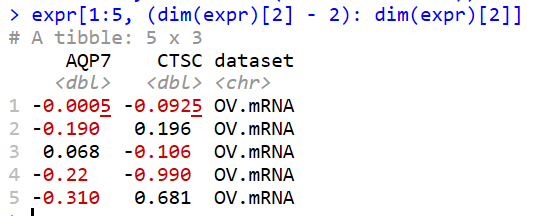
\includegraphics[height=4.5cm, width=8.5cm]{Yxq33as}
\caption{2}
\end{figure}


    \end{frame}

\subsection{Heterogeneous Analysis}
    \begin{frame}

    \begin{figure}[htbp]
\centering
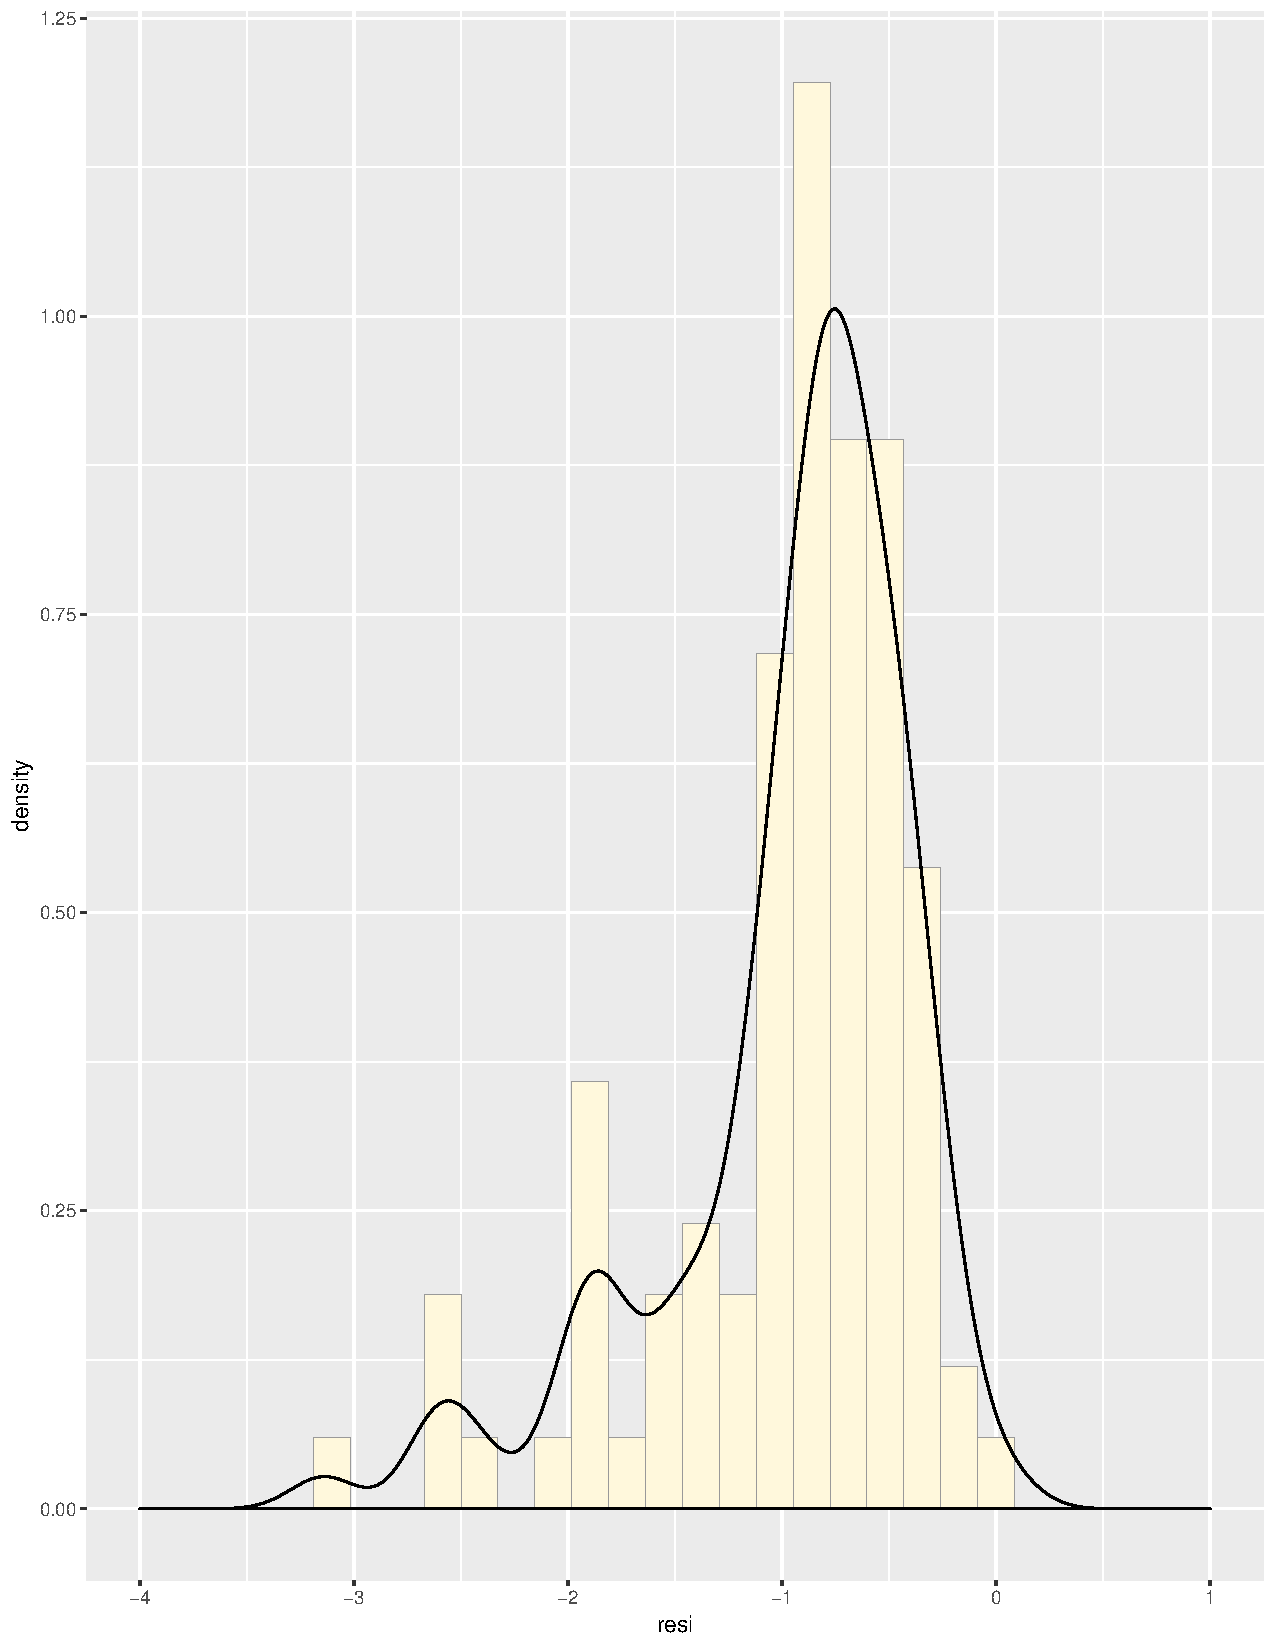
\includegraphics[height=5.5cm, width=8.5cm]{Rplot01}
\caption{4}
\end{figure}

    \end{frame}
    \section{Model and Algorithm}
    \subsection{Modelling}
    \begin{frame}
Assumed that $p\gg n$, we establish the subject-specified linear model
$$y_i=\mu_i+{\rm x}_i^T\beta+\epsilon_i, i=1,\dots,n$$
where $\beta=(\beta_1,\dots,\beta_p)^T$ is a $p-$dimension vector of the parameters.

And $\epsilon_i$ is error term independent with covariates ${\rm x}_i$ with
$$\mathbb{E}(\epsilon_i)=0, \mathbb{V}(\epsilon_i)=\sigma^2$$.
\end{frame}
\begin{frame}
Applied MCP[Zhang, 2010] to the diffrences of intercepts $\mu_i-\mu_j, 1\le i<\le j$and the parameters $\beta_k, k=1,\dots,p$, we can obtain
$$Q_n(\mu,\beta;\lambda,\omega)=\frac{1}{2}\sum_{i=1}^n(y_i-\mu_i-{\rm x}_i^T\beta)^2+\sum_{1\le i< j\le n}p_{\gamma}(|\mu_i-\mu_j|,\lambda)+\sum_{k=1}^pp_{\gamma}(|\beta_k|,\omega)$$
where
$$p_{\gamma}(t,\lambda)=\lambda\int_0^t(1-\frac{x}{\gamma\lambda})_+dx,\gamma>1$$
And the sign $(x)_+$ means that
$$(x)_+=\begin{cases}x,x>0\\0,x\le 0\end{cases}$$

\end{frame}

\begin{frame}
Define
$$\eta_{ij}=\mu_i-\mu_j$$
Denote
$$\eta = \{\eta_{ij},i<j\}^T$$
Then
$$\min S_n(\mu, \beta,\eta;\lambda,\omega)=\frac{1}{2}\sum_{i=1}^n(y_i-\mu_i-{\rm x}_i^T\beta)^2+\sum_{1\le i< j\le n}p_{\gamma}(|\eta_{ij}|,\lambda)+\sum_{k=1}^pp_{\gamma}(|\beta_k|,\omega)$$
$$s.t.\ \mu_i-\mu_j=\eta_{ij}$$
\end{frame}
\begin{frame}
Trough Augmented Lagrange multiplier method, we can obtain
$$L(\mu,\beta,\eta,\nu)=S_n(\mu,\eta,\beta)+\sum_{1\le i<j\le n}\nu_{ij}(\mu_i-\mu_j-\eta_{ij})+\frac{\vartheta}{2}\sum_{1\le i<j\le n}(\mu_i-\mu_j-\eta_{ij})^2$$
where $\vartheta$ is the penalty parameter and $\nu=\{\nu_{ij}\,i<j\}^T$ are Lagrange multipliers.
\end{frame}
\subsection{Computation}
\begin{frame}
\frametitle{Compute $\hat{\eta_{ij}}$}

$$L(\mu,\eta,\beta,\nu)=\sum_{1\le i<j\le n}\left\{\frac{\vartheta}{2}(\mu_i-\mu_j+\vartheta^{-1}\nu_{ij}-\eta_{ij})^2+p_{\gamma}(|\eta_{ij}|,\lambda)\right\}+C_1$$
Therefore
$$\frac{\vartheta}{2}(\mu_i-\mu_j+\vartheta^{-1}\nu_{ij}-\eta_{ij})^2+p_{\gamma}(|\eta_{ij}|,\lambda)$$
Let
$$\delta_{ij}=\mu_i-\mu_j+\vartheta^{-1}\nu_{ij}$$
Denote
$$\delta = \{\delta_{ij},i<j\}^T$$
\end{frame}
\begin{frame}
We can obtain given $\delta^{(m+1)}$ at the $m-$step, we can update $\eta^{(m+1)}$ whose elements are the minimizer of (2.7) as
$$\eta^{(m+1)}=\begin{cases}\frac{ST(\delta^{(m+1)},\lambda/\vartheta)}{1-1/\gamma\vartheta},|\delta^{(m+1)}|\le \gamma\lambda\\ \delta^{(m+1)}, |\delta^{(m+1)}|>\gamma\lambda\end{cases}$$
where $ST(t,\lambda)=sign(t)(|t|-\lambda)_+$ is the soft-therosholding function. And given $\nu^{(m)}$ at the $m-$step and$\mu^{(m+1)}$ at the $(m+1)-$step, the update $\delta^{(m+1)}$ is $$\delta^{(m+1)}=\Delta\mu^{(m+1)}-\frac{1}{\vartheta}\nu^{(m)}$$
where$\Delta=\{e_i-e_j,i<j\}^T, e_i$ is a $n$-dimension vector with the $i-$th component 1 and others 0.
\end{frame}
\begin{frame}
\frametitle{Compute $\hat{\mu}$}

\begin{align*}L(\mu,\eta,\beta,\nu)=&\frac{1}{2}\sum_{i=1}^n(y_i-\mu_i-{\rm x}_i^T\beta)^2+\sum_{1\le i<j\le n}\nu_{ij}(\mu_i-\mu_j-\eta_{ij})\\
&+\frac{\vartheta}{2}\sum_{1\le i<j\le n}(\mu_i-\mu_j-\eta_{ij})^2+C_2\end{align*}
Then
$$\begin{aligned} L(\mu,\eta,\beta,\nu)&=\frac{1}{2}\|y-\mu-X\beta\|^2+\frac{\vartheta}{2}\sum_{1\le i<j\le n}(\mu_i-\mu_j-\eta_{ij}+\vartheta^{-1}\nu_{ij})^2+C_3\\
&=\frac{1}{2}\|y-\mu-X\beta\|^2+\frac{\vartheta}{2}\sum_{1\le i<j\le n}\left\{(e_i-e_j)\mu-\eta_{ij}+\vartheta^{-1}\nu_{ij}\right\}^2+C_3\\
&=\frac{1}{2}\|y-\mu-X\beta\|^2+\frac{\vartheta}{2}\|\Delta\mu-\eta+\vartheta^{-1}\nu\|^2+C_3
\end{aligned}$$
\end{frame}
\begin{frame}
Let
$$\frac{\partial L(\mu,\eta,\beta,\nu)}{\partial \mu}=-(y-\mu-X\beta)+\vartheta\Delta^T(\Delta\mu-\eta+\vartheta^{-1}\nu)=0$$
Given $\eta^{(m)},\nu^{(m)},\beta^{(m)}$ at the $m-$step, we obtain
$$\mu^{(m+1)}=(E_{n\times n}+\vartheta\Delta^T\Delta)^{-1}(\vartheta\Delta^T\eta^{(m)}-\Delta^T\nu^{(m)}+y-X\beta^{(m)})$$
where $E_{n\times n}$ is $n$-dimension unit matrix.
\end{frame}

\begin{frame}
\frametitle{Compute $\hat{\beta}$}
\begin{align*} L(\mu,\eta,\beta,\nu)&=\frac{1}{2}\sum_{i=1}^n(y_i-\mu_i-{\rm x}_i^T\beta)^2+\sum_{k=1}^p p_{\gamma}(|\beta_k|,\omega)+C_4\\
&=\frac{1}{2}\|y-\mu-X\beta\|^2+\sum_{k=1}^p p_{\gamma}(|\beta_k|,\omega)+C_4
\end{align*}
Let $\tilde{y}=y-\mu$, then (10) is equivalent to
$$L(\mu,\eta,\beta,\nu)=\frac{1}{2}\|\tilde{y}-X\beta\|^2+\sum_{l=1}^pp_{\gamma}(|\beta_l|,\omega)+C_4$$
\end{frame}

\begin{frame}
The solution of (2.11) is given by Patrick B.(2011), that is, given $\mu^{(m+1)}$ at the $(m+1)-$step, the update is
$$\beta^{(m+1)}=\begin{cases}\frac{ST(n^{-1}X^T\tilde{y}^{(m+1)},\omega)}{1-1/\gamma},|n^{-1}X^T\tilde{y}^{(m+1)}|\le\gamma\omega\\ n^{-1}X^T\tilde{y}^{(m+1)},|n^{-1}X^T\tilde{y}^{(m+1)}|>\gamma\omega\end{cases}$$
where $\tilde{y}^{(m+1)}=y-\mu^{(m+1)}$. And this can be estimated in the ncvreg R-package by Breheny P. and Huang J. (2011).
\end{frame}
\subsection{Algorithm}
\begin{frame}
\frametitle{Stopping criterion}
Define
\begin{align*}D^{(m+1)}_{\mu} &= \left\{(\Delta\mu^{(m+1)}-\eta^{(m+1)})^T(\Delta\mu^{(m+1)}-\eta^{(m+1)})\right\}^{\frac{1}{2}}\\
D_{\beta}^{(m+1)}&=\left\{ (\beta^{(m+1)}-\beta^{(m)})^T(\beta^{(m+1)}-\beta^{(m)})\right\}^{\frac{1}{2}}
\end{align*}
Let $\|s\|_w$ be the weighted average norm by weighting the values of norms applied to every elements of $s$. In this paper, we terminate the iteraction when $\|D^{(m+1)}\|_w$ is less than a pre-defined tolerance, where $D^{(m+1)}=(D_{\mu}^{(m+1)},D_{\beta}^{(m+1)})$,

and
 $$\|D^{(m+1)}\|_w=\omega_0\|D_{\mu}^{(m+1)}\|+\omega_1\|D_{\beta}^{(m+1)}\|, \omega_0+\omega_1=1$$.
\end{frame}

\begin{frame}
\frametitle{Algorithm}
By ADMM, we can obtain the iteration function of $\nu$ is
$$\nu^{(m+1)}=\nu^{(m)}+\vartheta(\Delta\mu_{(m+1)}-\eta^{(m+1)})$$
Therefore, the algorithm is as follows.


\end{frame}
\begin{frame}

\frametitle{Selection of tunig parameters}

$$BIC(\lambda,\omega)=\log\left[\frac{\sum_{i=1}^n\left(y_i-\hat{\mu}_i(\lambda,\omega)-{\rm x}_i^T\hat{\beta}(\lambda,\omega)\right)^2}{n}\right]+C_n\frac{\log n}{n}\left(\hat{K}(\lambda,\omega)+p\right)$$
where $C_n$ is a positive numbers depending on sample size $n$. With $C_n=1$, the revised BIC is indeed the traditional BIC. Wang, LI, and Leng(2009) suggests
$$C_n=c\log(\log(n+p))$$
where $c$ is a positive number. The pair $(\lambda,\omega)$ minimized $BIC(\lambda,\omega)$ is applied to the model fit.

  \end{frame}
\section{Results}
\begin{frame}
    \begin{figure}[htbp]
\centering
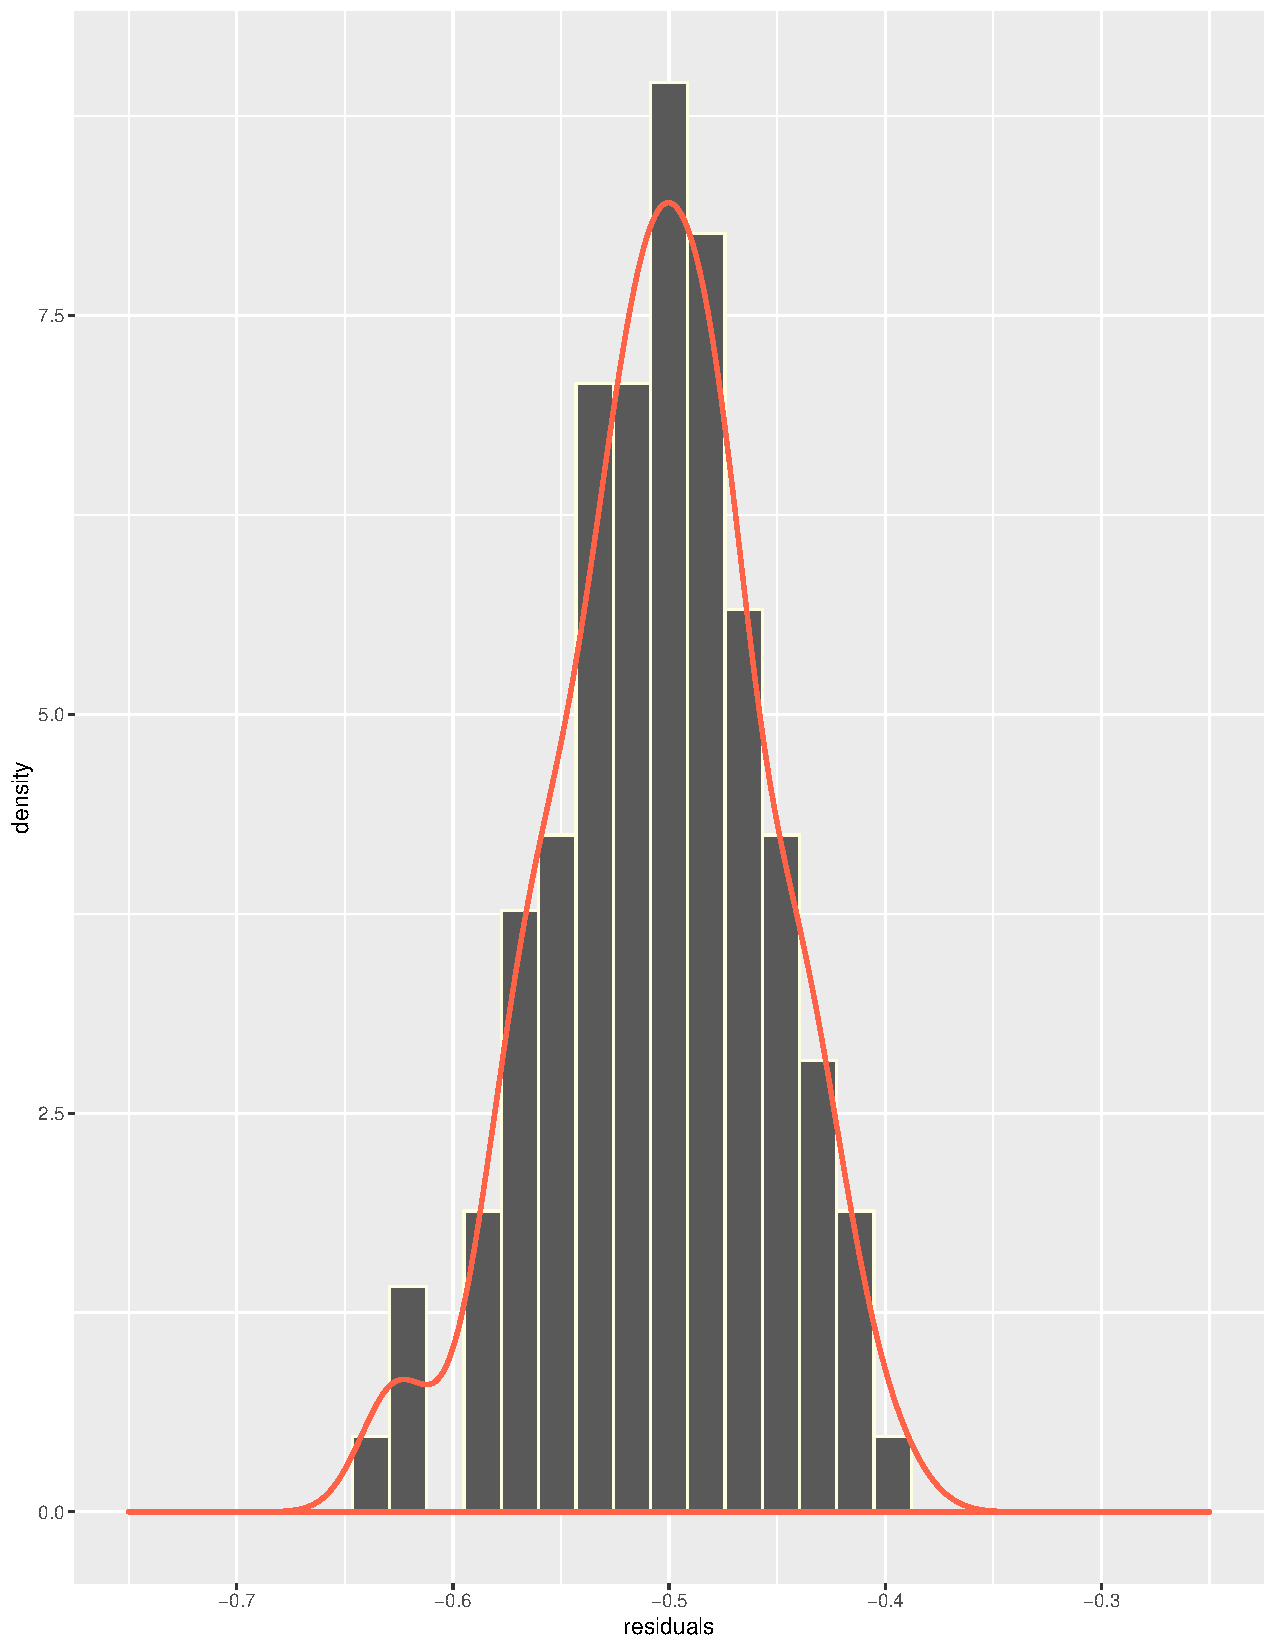
\includegraphics[height=5.5cm, width=8.5cm]{Rplot-2}
\caption{group 1}
\end{figure}


\end{frame}
\begin{frame}

\begin{figure}[htbp]
\centering
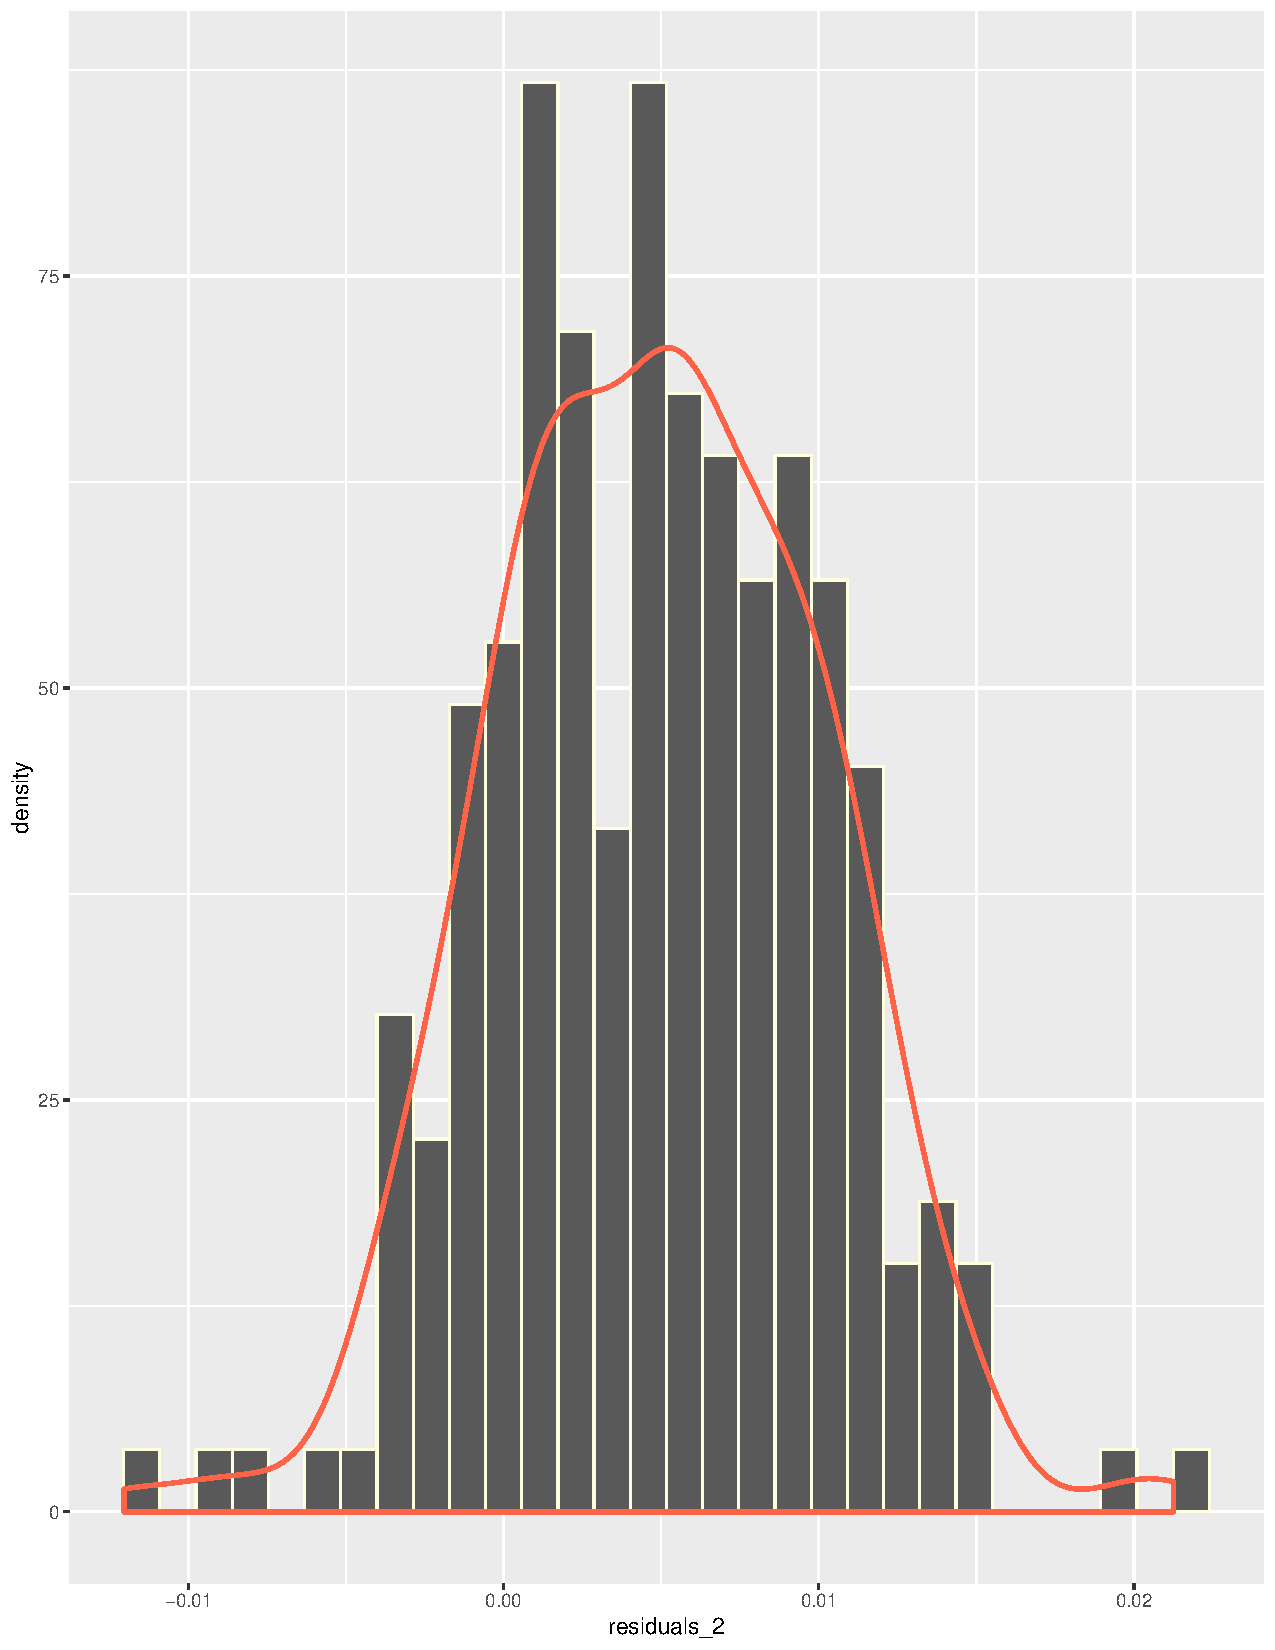
\includegraphics[height=5.5cm, width=8.5cm]{Rplot_3}
\caption{group 2}
\end{figure}
\end{frame}

\begin{frame}
\begin{figure}[htbp]
\centering
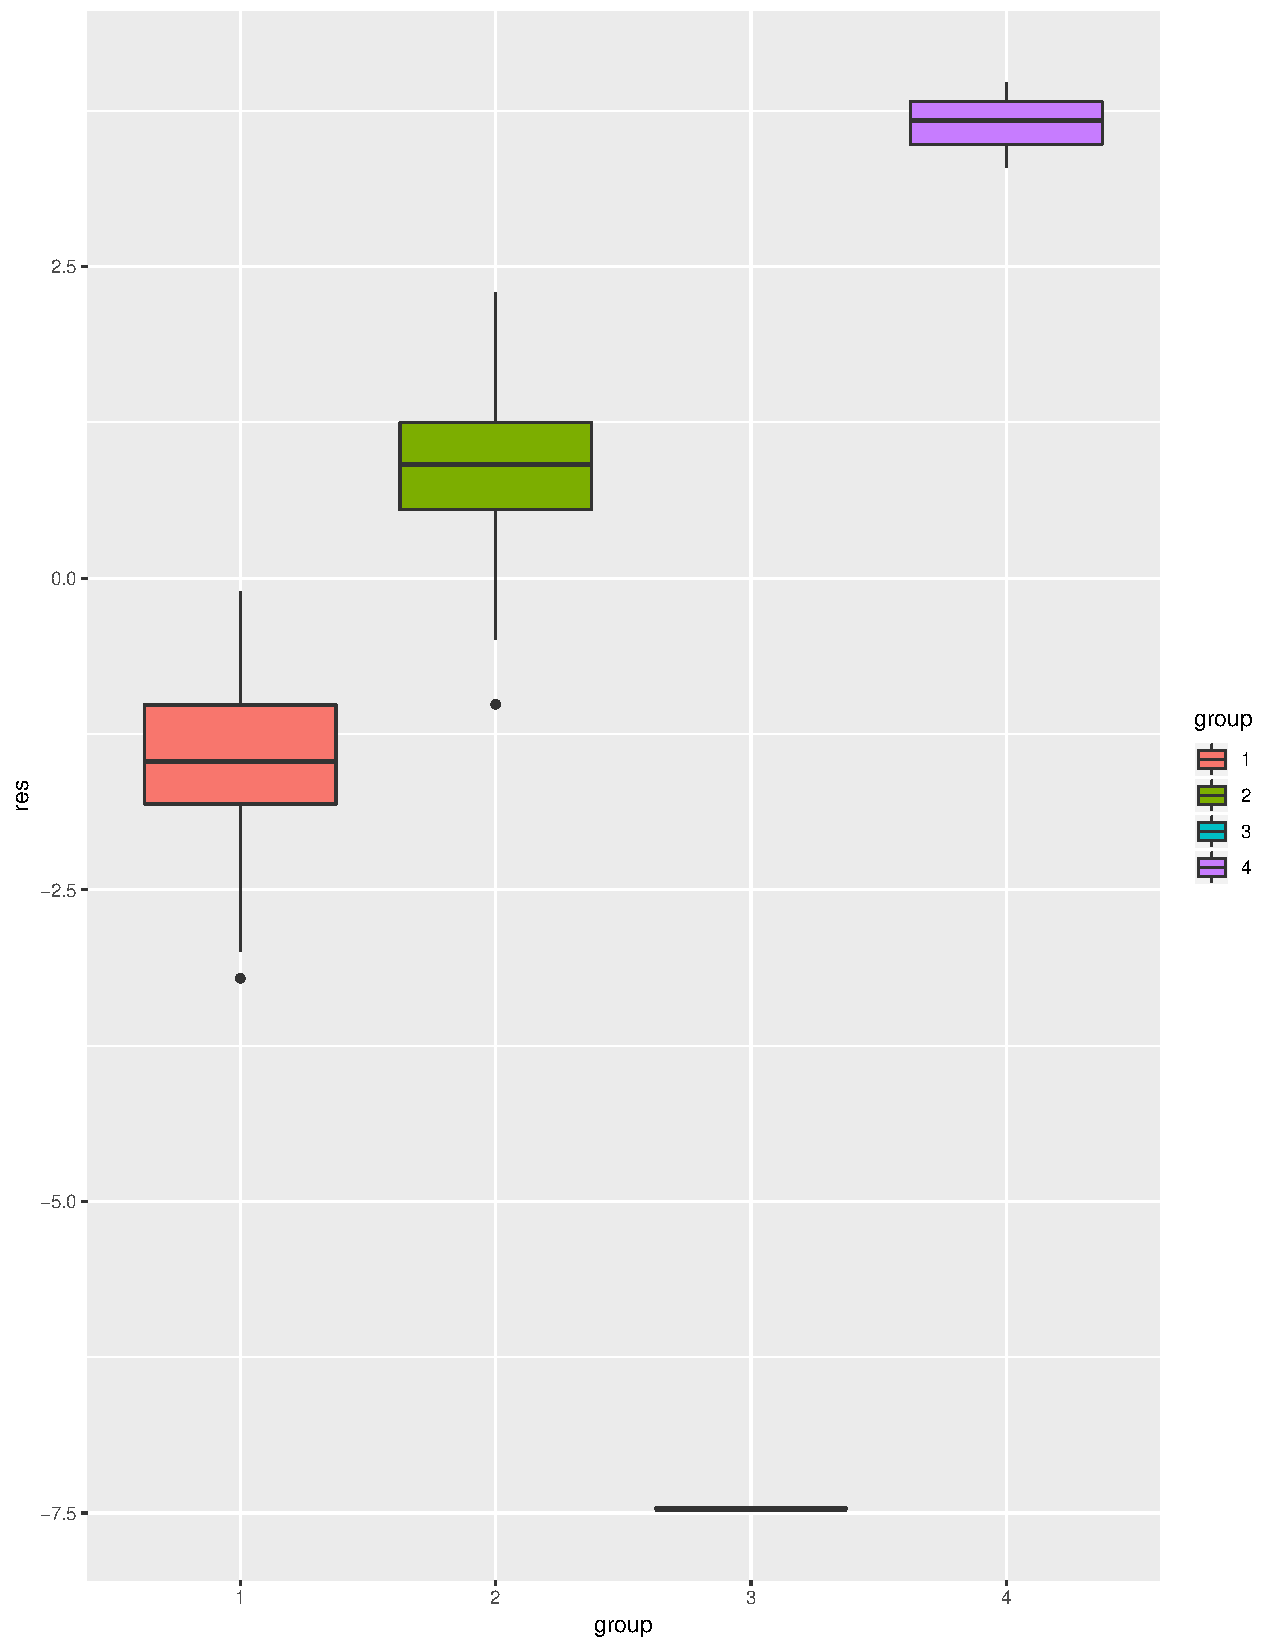
\includegraphics[height=5.5cm, width=8.5cm]{Rplot-4}
\caption{Boxplot of the divided groups}
\end{figure}

\end{frame}

    \begin{frame}
    \frametitle{Thanks}
    Thank you!
    \end{frame}
\end{CJK*}
\end{document}
